\section{Interannual response to ENSO variability}

In this section, the interannual response of epipelagics to ENSO variability is investigated using covariance analysis, as done in section \ref{sec:sst}. 
The focus will be first laid on vertically integrated 
fish biomass, in order to have a spatial vue of the response. Then, the response of the fish biomass as a function of longitude and depth will be investigated.\\

For the sake of simplicity, the focus will be laid on three size classes: 3cm, representing small fishes, 20cm, representing intermediate sizes, and 90 cm, representing large individuals. These sizes are also
representative of the sizes of tuna target species within the region.\\

\subsection{Vertically integrated biomass}

The left panels of figure \ref{fig:mean-cov-ape} show the yearly mean vertically integrated fish biomass ($J.m^{-2}$) over the entire simulation for the three different size classes. For small sizes (figure \ref{fig:mean-cov-ape}a), the fish biomass is concentrated at around 10\degree S and 10 \degree N in the central Pacific and close to 0the equator in the western Pacific. High biomass concentration is also found east of 90\degree W, off the coasts of Chili. As size increases, the equatorial "blue spot" extends meridionnally and to the west. This pattern is mostly driven by the active and passive advection of fishes in the Apecosm model (\warn{REF}). Without advection, the biomass will be concentrated at the equator, where the plankton concentration is the maximum. 

\begin{figure}[h!]
    \centering
    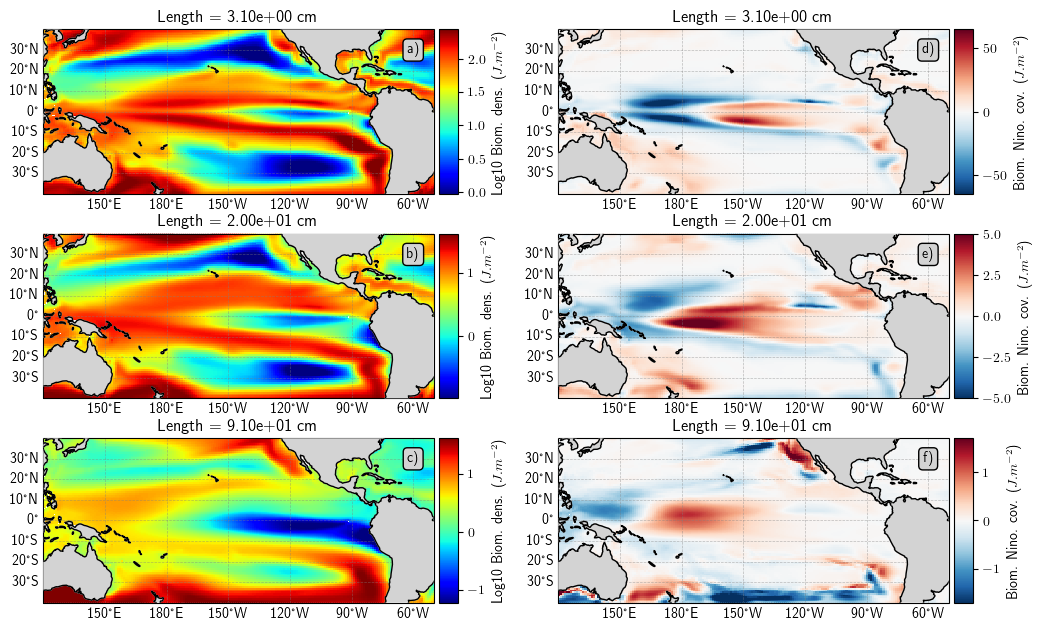
\includegraphics[width=\textwidth]{covariance_mean_epi.png}
    \caption{Yearly average of biomass density (left panel, log-scale, $J.m^{-2}$) and 
    covariance between the yearly average biomass density and the winter-average ONI index (right panels, $J.m^{-2}$)}
    \label{fig:mean-cov-ape}
\end{figure}

Covariance maps between vertically integrated fish biomass and the winter ONI index are shown in the right panels of figure \ref{fig:mean-cov-ape}. 
Small epipelagics show negative anomalies in the Western Equatorial Pacific and positive anomalies in the Central Equatorial Pacific. This pattern can be interpreted as an eastern displacement of the mean biomass in the Western Pacific.\\

Similar dipolar patterns are also obtained for intermediate and large sizes, but the anomalies westward shifted as size increases. This can be interpreted, as for small sizes, by a westward shift of fish biomass during positive \nino\ phases.\\

\subsection{Equatorial biomass profile}

The yearly mean equatorial profile of fish biomass density, obtained by averaging the 3D biomass density between 2\degree S and 2\degree N, 
is shown figure \ref{fig:mean-forage}, for day (left panels) and night (right panels). Small size classes (0-3cm and 3cm-20cm) show similar 
patterns during both nights and days. In the east, the fish biomass is concentrated at the surface, betweem 0 and 25m. In the west, small epipelagics
are found down to 75m. For larger sizes (20cm-90cm and 90cm-200cm), the biomass vertical distribution changes between day and night. During the day, the equatorial fish biomass is concentrated in the western Pacific at around 150\degree E. During day-time, the biomass is concentrated at around 50m, while during night-time, the biomass is equally distributed between the surface and 125m.\\

\begin{figure}[h!]
    \centering	
    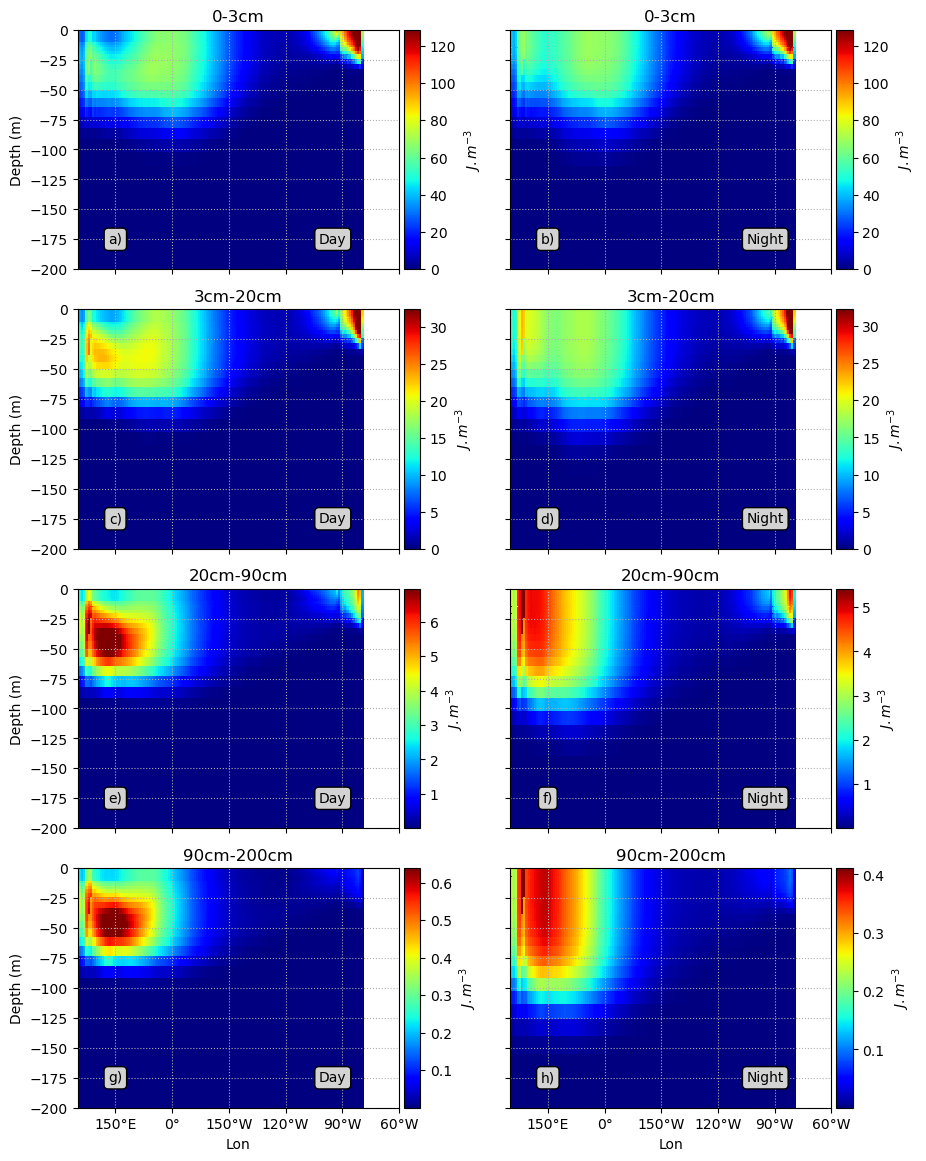
\includegraphics[width=\textwidth]{forage_mean.png}
	\caption{Mean epipelagic biomass density integrated over 2\degree S and 2\degree N}
    \label{fig:mean-forage}
\end{figure}

\begin{figure}[h!]
    \centering
    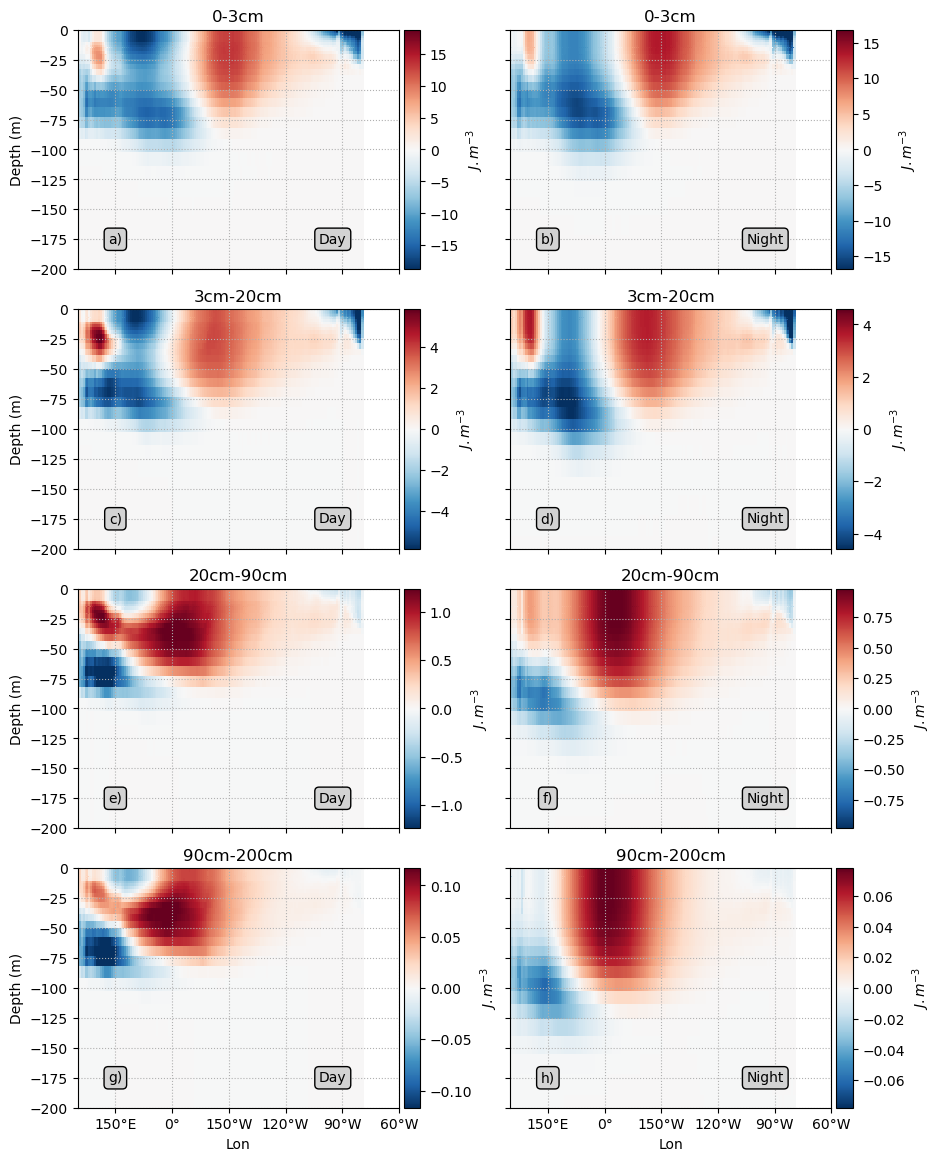
\includegraphics[width=\textwidth]{forage_covariance.png}
	\caption{Covariance between yearly anomalies of epipelagic biomass density integrated over 2\degree S and 2\degree N and the winter ONI index.}
    \label{fig:covariance-forage}
\end{figure}

The covariance between the equatorial profil of yearly fish biomass distribution and the winter ONI index is shown in figure \ref{fig:covariance-forage}. As for the mean profile, there is no differences between day and night. The covariance patterns shows a tripolar pattern, with negative anomalies in the western and eastern Pacific, and positive anomalies in the central Pacific.\\

Large sizes show a dipolar covariance, with positive anomalies near the equator, and negative anomalies in the western Pacific. 
During the day, the negative anomalies are situated at arount 75m but extends from the surface to 100m during the day. The positive anomalies are concentrated between 25 and 75m during the day, but extends from the surface to 100m during the night.

\subsection{Transient response to ENSO variability}

In order to analyse the transient response to ENSO variability, lead-lag covariance analysis has been performed. The monthly vertically integrated fish biomass has been averaged between 2\degS{} and 2\degN{}. Then, monthly anomalies has been computed by removing the mean seasonaly cycle. Finally, lead-lag covariance has been applied between the fish biomass anomalies and the monthly ONI index (figure \ref{fig:hov-cov-oope}).

\begin{figure}[h!]
    \centering
    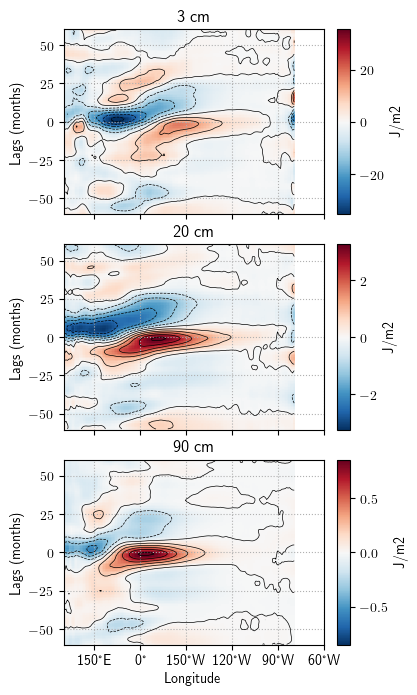
\includegraphics[scale=0.5]{equatorial_covariance_OOPE.png}
    \caption{Lead-lag covariance between the monthly ONI index and the vertically integrated fish biomass. The ONI leads for positive lags.}
    \label{fig:hov-cov-oope}
\end{figure}

The covariance patterns is very similar for the three size classes, with
 positive anomalies in the central Pacific and negative
anomalies in the Western Pacific at lag 0, which is consistent 
with the annual covariance shown in figure \ref{fig:mean-cov-ape} (right panels). However, the positive anomalies are westward shifted as size increases, with positive anomalies at around 150\degW{} for smaller sizes and close to the dateline for bigger sizes. \warn{Explain why}. It can be noticed that the positive anomalies does not seem to show any propagation over time, contrary to the negative anomalies. This is especially clear for the 20 cm size class, for which the negative anomalies are centerred at around 150\degE{} at lag 0 and reach 150\degW after 20 months.

 


%\subsection{Interannual response to ENSO variability}
%
%\subsection{Transient biological response to \nino}
%
%\begin{figure}[h!]
%    \centering
%    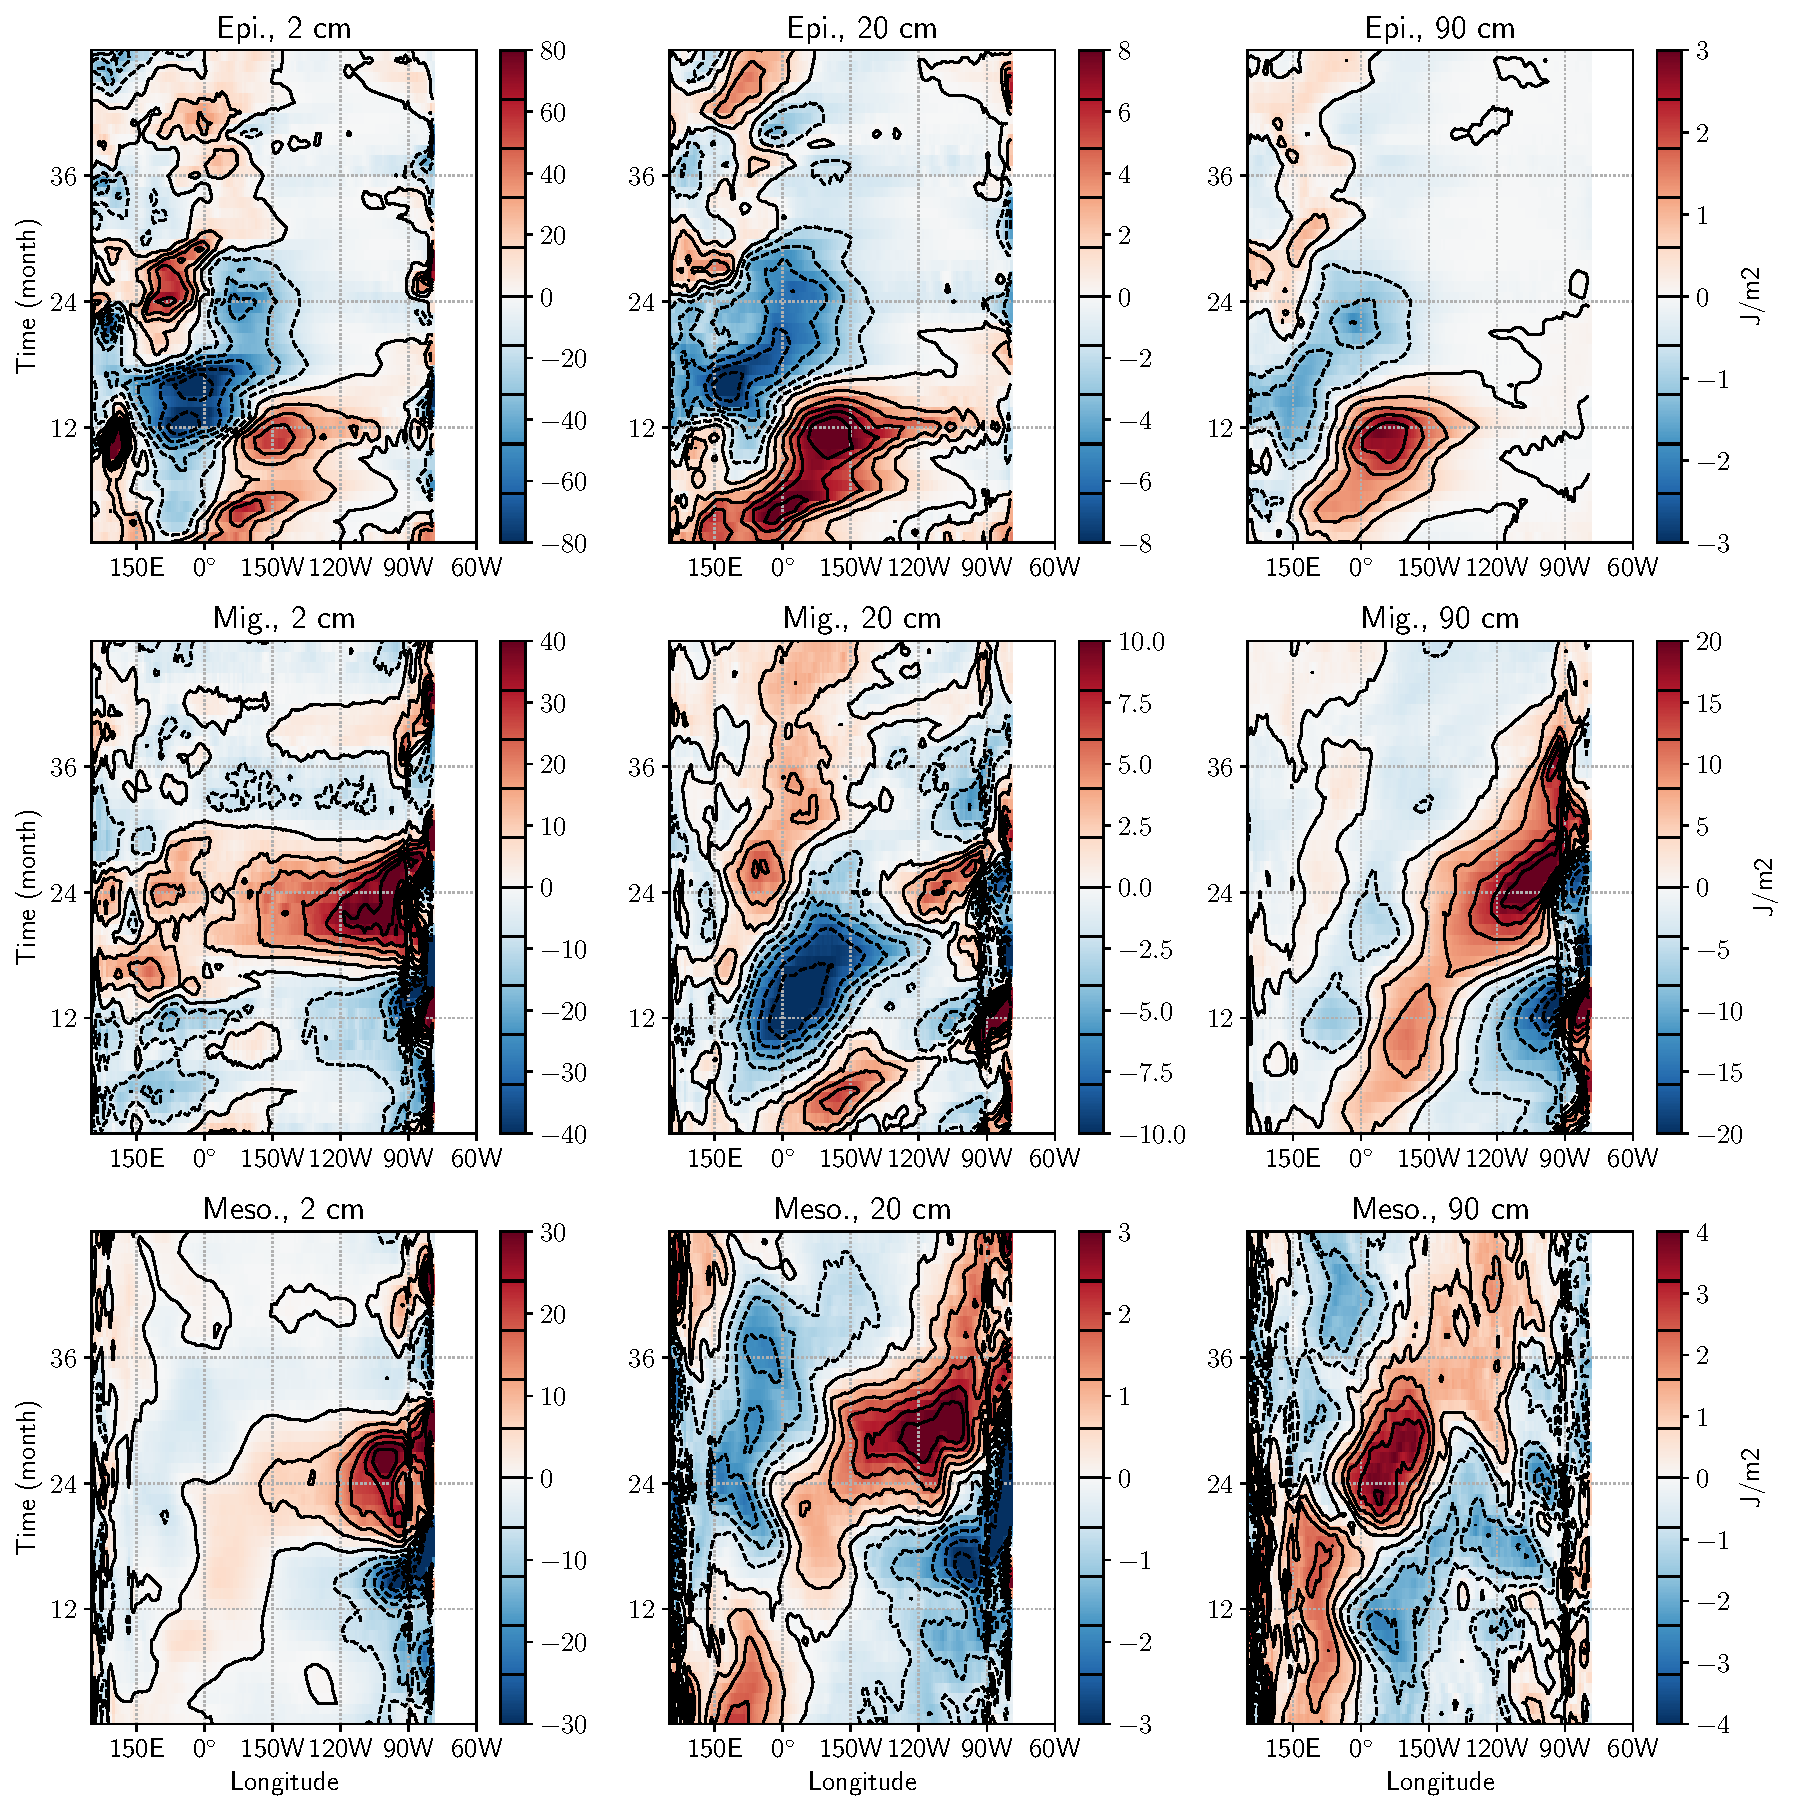
\includegraphics[scale=0.5] {debugged_corr_mask_hovmoller_composites_OOPE}
%    \caption{Composites of \hov\ diagram composite of fish biomass density ($J.m^{-2}$) along the equatorial Pacific ocean.}
%    \label{fig:hov-oope}
%\end{figure}

\clearpage
